\documentclass[11pt,a4paper,UKenglish]{article}
\usepackage[utf8]{inputenc}           %% ... or latin1
\usepackage[T1]{fontenc,url}
\usepackage{textcomp,csquotes,varioref,graphicx}
\usepackage{gensymb}
\usepackage[english]{babel}

\usepackage[top=1in]{geometry}
\usepackage{float}
\usepackage[hidelinks,colorlinks]{hyperref} % trykkbar referering
\usepackage[all]{hypcap} % ref til starten av referansen
\usepackage{todonotes} % for kladd

\usepackage{marginnote}
\usepackage[backend=biber,style=numeric-comp]{biblatex}
\addbibresource{text_seg.bib}
% \addbibresource{bib.bib}

\usepackage{ifikompendium/ifikompendiumforside}

\title{UNIK4690 Project}
\subtitle{Text Recognition}
\author{
  Akhsarbek Gozoev  - akhsarbg \\
  Sadegh Hoseinpoor - sadeghh\\
  Key Lung Wong - keylw
}
\begin{document}
\ififorside[kind={Report}]

\newpage
\tableofcontents
\newpage
\section{Introduction}
\label{sec:Introduction}
\noindent \\ This report is divided into 5 sections\todo{refrence and recognition
should maybe be divided?}. In Section~\ref{sec:Introduction}, we introduce the
Report and how the report is organized. Section~\ref{sec:Project description} is
where we describe the project and where we present our initial thoughts and
approach on how solve our problem. In Section~\ref{sec:Project review} we
review our approach and present how we solved the problem, methods we used and
changes which had to be performed. In Section~\ref{sec:Project conclusion} we
present thoughts on the project and what could be done differently,
difficulties that we faced and, a step by step tutorial on how to run our
software. Section~\ref{sec:Recognition} includes third party material we have used.


\newpage

\section{Project description}
\label{sec:Project description}
\textbf{The purpose of the software is to recognize text from any
surface with uneven lighting. Hence this falls under the ``Optical
character recognition'' (OCR) problem}

\noindent \\ As OCRs are still a challenging task even for companies like
Google, ref. reader to Googles OCR translator application on smartphones;
``Translate'', drawbacks such as; difficulty finding all the text on the photo
because of lighting, noise etc., therefore we will have to limit our software
significantly.


\subsection{Initial limitations}
\begin{itemize}
 \item{English alphabet + numbers [0-9]}
 \item{Homogeneous background}
 \item{Skew free text}
 \item{Computer printed text}
\end{itemize}

\subsection{Project components}
The group have come to the conclusion that the OCR software has 3 main
components to it.
\begin{enumerate}
 \item{\textit{Text segmentation}}
 \begin{itemize}
  \item{Finding text on an image and returning the text segments}
 \end{itemize}
 \item{\textit{Preprocessing}}
 \begin{itemize}
  \item{Do preprocessing on the segmented text; rotation, symbol segmentation,
  etc.. (preprocessing from its definition, should be done first, however
  because of simplification we assume we manage to segment out text first.)}
 \end{itemize}
 \item{\textit{Classification}}
 \begin{itemize}
  \item{Classification of the symbols}
 \end{itemize}
\end{enumerate}
\noindent \\ Additionally there is one more very important component for this
OCR software to work, \textit{\textbf{labeled data}}. Even though one might not
need to code for this part, a good pool of labeled data is needed to be able to
classify symbols. More on this later.
\noindent \\ (4. \textit{Data classification - Gathering labeled data to train a classification algorithm})

\subsection{Component description}
This section we will describe our thoughts on how we plan to solve each
component, in the form of algorithms, APIs, and datasets. Note that this is our
initial thoughts, not necessary the solution we will end up implementing.
Additionally, as we want to test proof-of-concept while we are coding, we will
be making several simplifications. Relevant simplifications will be described
further under each component.


\subsubsection{Text Segmentation}\label{Component_Descripton:Text_segmentation}
\noindent \\ \textbf{Description}
\noindent \\ We where uncertain on how to do this part when we initial started the project. We ended up looking for a lot of different ways to do this part. We ended up trying 3 different approaches with mix result.
\begin{enumerate}
  \item Simple image analysis technics, using Otsu thresholding and Morphology.
  \item OpenCv implementation of Scene Text Detection.
  \item Stroke Width Transform(SWT) to detect text in natural images.
\end{enumerate}

\noindent \\ \textbf{Approach 1: Simple Image Analysis Technics}
\noindent \\ We was inspired by the this online blog \href{https://www.danvk.org/2015/01/07/finding-blocks-of-text-in-an-image-using-python-opencv-and-numpy.html}{Source}\cite{_finding_????}. We simplified the original approach where we only look at an image with text. The approach is then simply do an Otsu Thresholding and then morphological Closing to connect component. After that we used OpenCv FindContours method to find the contour of the different text regions. FindContours in OpenCv uses the algorithm proposed by Suzuki, S. and Abe, K. 1985\cite{suzuki_topological_????}.

\noindent \\ \textbf{Approach 2: OpenCv Scene Text Detection}
\noindent \\ OpenCV have it own Text Scene Detection. The approach of this algorithm is to detect text in scene using Classifier and Components Tree, propose by Lukás Neumann \& Jiri Matas \cite{neumann_real-time_2012}.

\noindent \\ \textbf{Approach 3: Stroke Width Transform}
\noindent \\ We also found Stroke Width Transform to do Text Segmentation\cite{epshtein_stroke_2010}. Similar to OpenCv Scene text detection, it looks for text in natural images. The approach of the Algorithm is to calculate the different stroke length of the different elements in the image. Based on the stroke length, evaluate if it is a text element or not. The concept was relative simple to grasp. The implementation, in the other hand, was quite difficult to implement. We will look at the full implementation later in.

\subsubsection{Preprocessing}
\noindent \\ \textbf{Description}
\noindent \\ Definition of preprocessing; the act of readying the data for
further use, in our case for classification. \par
The specification of how the format of the image should be is not in our hands,
as we will use datasets from third parties. We have to make the format and
type of our input the same as the datasets. Other than the specifications we
also need to take into account the spatial characteristics of the data, as we
want the chance of the data correctly classified as high as possible. Such as
background-foreground intensity, lighting, rotation, location of the
character, etc.. \par

\noindent \\ \textbf{Limitation - proof-of-concept}
\noindent \\ We will here limit our input data to only include grey-level
images with rotation. As we progress further into the project we will include
more aspects of a realistic image.

\noindent \\ \textbf{Challenges}
\begin{itemize}
 \item{Rotated text}
 \begin{itemize}
  \item{Hough transform is a valid solution to this problem. Finding the angle
  of the lines and then rotate the text segments accordingly.}
 \end{itemize}
 \item{Line segmentation}
 \begin{itemize}
  \item{Projection histograms allows us to find where the lines start and end,
  both vertically and horizontally.}
 \end{itemize}
 \item{Character segmentation}
 \begin{itemize}
  \item{We can use projection histogram here as well, however one line at a
  time. This way we can find out where each symbol starts and end.}
 \end{itemize}
\end{itemize}


\subsubsection{Classification}
\noindent \\ \textbf{Description}
\noindent \\ At this point because of available knowledge and the interest in
Convolutional Neural network (CNN), we ended up trying to solve this part
both with a CNN, and a Multilayer Perceptron (MLP or Deep neural network (DNN)).
Illustration of each of the architectures are available, CNN Figure~\ref{fig:CNN_architecture},
and the MLP network Figure~\ref{fig:neural_net2}. \par
To avoid inventing the wheel again, we will use the TensorFlow API, the low
level API will suffice for the MLP, and the high level API we will try for the
CNN.

\noindent \\ \textbf{Deep Neural Network}
\noindent \\ Multilayer perceptron neural networks are relatively straight
forward to code, however the challenging part is to decide on good
hyper-parameters and to not overfit our network. \par
Research has shown that the choices of parameters can have huge effects on
the error rate through empirical testing. As empirical testing has shown that
some combinations of parameters are better than others, we will also use the
same method to find decent values on several of the hyper-parameters. More on
this below, where a short description of the hyper-parameters follow. \par
One obvious disadvantage we might face by using MLP is that slight spatial
change on where in the image the characters are located, might lead to
characters classified differently. This is because there is no spatial
connections on a MLP.

\begin{figure}[H]
  \centering
  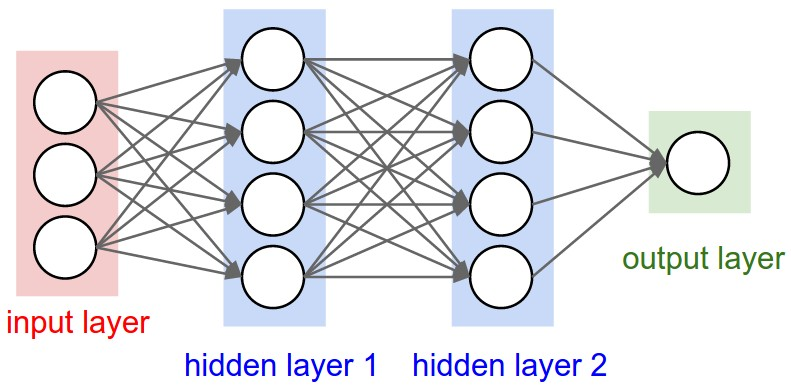
\includegraphics[height=4cm]{res/neural_net2.jpeg}
  \caption{MLP Neural network \href{http://cs231n.github.io/neural-networks-1/}{Source}}
  \label{fig:neural_net2}
\end{figure}


\noindent \\
\noindent \\ \textbf{Hyper-parameters}
\begin{itemize}
 \item{Number of hidden layers}
 \begin{itemize}
  \item{Layers decide how well the software can define the decision borders.
  Hence increase in layers can have a positive effect, there are also cons with
  the amount of layers. The more layers, the greater the computational power
  needed to train the system. We will be using the empirical method to decide
  how many layers we need}
 \end{itemize}
 \item{Number of nodes in each hidden layer}
 \begin{itemize}
  \item{Nodes in each hidden layer has the same effect as the number of hidden
  layers, hence the same applies for this hyper-parameter. }
 \end{itemize}
 \item{Activation functions}
 \begin{itemize}
  \item{The activation function decides which combination of nodes, with their
  signals, are allowed to propagate through the network. Here we will be using
  the \textit{rectified linear unit} (RELU) activation function. This is an
  activation function that allows propagation if the signal is positive,
  otherwise it will forward a zero. The reason for choosing this activation
  function is because this function handles the \textit{vanishing gradient
  problem} better than sigmoid and a tanh activation functions. More on
  vanishing gradient problem under ``optimization function''.}
 \end{itemize}
 \item{Loss function}
 \begin{itemize}
  \item{The loss function describes how far off the predicted class of the
  character is from the real class. In our case since we have multiple
  classes and we are going to use \textit{softmax regression} as the output
  layer, we also will be using the \textit{cross-entropy loss function}.}
 \end{itemize}
 \item{Optimization function}
 \begin{itemize}
  \item{The backpropogation will train the weights by Gradient Decent
  Optimization. However as training with several thousand examples, and then
  optimizing the weights and run the training process, is too costly resource
  wise, we will have to implement the \textit{mini-batch gradient decent
  optimizations}. Same principle as gradient decent optimization, but this way
  we will find the gradient decent for each batch. As long as these batches are
  randomly chosen, and the sizes are large enough, (we will be using 100 as
  batch size), these will represent the entire dataset well enough.}
 \end{itemize}
 \item{Learning rate}
 \begin{itemize}
  \item{Learning rate is a scalar that decides how large the steps towards
  the gradient minimum will be, for the weights. Choosing too small of a
  learning-rate we might risk not reaching the bottom of the graph, we also
  might get stuck in a local minimum. Choosing too large of a learning rate
  we might risk never settle down on a minimum. \par
  For the learning rate we will be using the empirical method too.}
 \end{itemize}
 \item{Initialization of the weights and biases}
 \begin{itemize}
  \item{Initialization of the weights also seems to be of importance,
  researchers have found out. This is obvious, as for example setting all the
  weights to zero, would of course lead to a network with very few active
  nodes. \par
  We will be using the initialization of zeros for the biases, not any
  apparent reason. Based on our research, it seems people have gotten decent
  results when using this initialization. For the weights we will be using a
  gaussian distribution, mean=0, standard deviation=1. Again this is also
  something that we have read should be a good initialization for the weights,
  no other reason.}
 \end{itemize}
 \item{Number of epochs}
 \begin{itemize}
  \item{Number of epochs are only relevant when we have a small number of
  dataset. When we have a small dataset we might want to run the software on
  the same dataset several times. This might result in overfitting the software
  to the dataset, therefore it is really important to be careful of the number of
  epochs, in cases with small datasets.}
 \end{itemize}
\end{itemize}


\noindent \\ \textbf{Convolutional Neural Network}
\noindent \\ Convolutional neural networks are especially good for image
classification, because they take local spatial connections into account when
they classify. This way it doesn't matter where in the image our
object/character is it will be able to recognize it, same yields for rotation,
as the CNN classifies based on local spatial connections it doesn't matter if
the object is rotated. Hence the classification would be even more robust
compared to the MLP. \par
The basic idea of a CNN is somewhat understood, but the algorithms and how to
implement it is still not 100\% grasped. Hence because of lack of knowledge,
trying to solve the classification problem with a CNN will mostly be done
by researching and trying to solve it as it unfolds.

\begin{figure}[H]
  \centering
  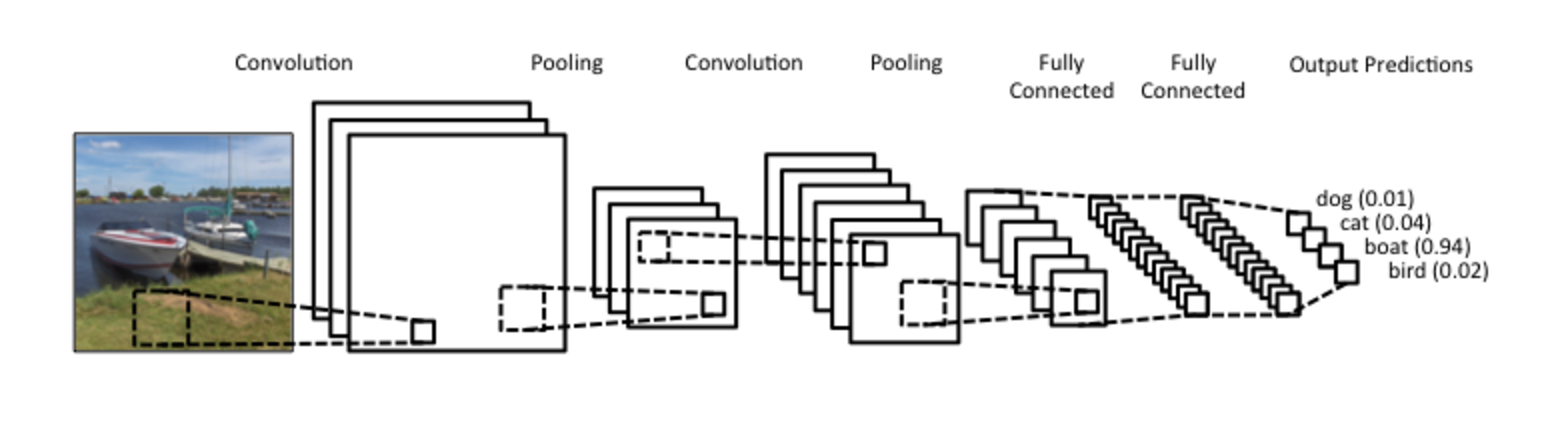
\includegraphics[height=4cm]{res/CNN_architecture.png}
  \caption{Convolutional Neural network \href{ http://www.wildml.com/2015/11/understanding-convolutional-neural-networks-for-nlp/}{Source}}
  \label{fig:CNN_architecture}
\end{figure}

\noindent \\ \textbf{CNN - Basics}
\begin{itemize}
 \item{Convolutional layer}
 \begin{itemize}
  \item{This layer consists of several filters/kernels that are convolved over
  the image and based on how many filters one uses, the same amount of feature
  images are made. The purpose of the filters are to grasp some spatial
  characteristics of the image, and make it available for further processing.
  The filters here correspond to the weights in the MLP, these are first
  initialized at random (or with a smart initialization method), then these
  will be updated as the network is trained. Some features that the filters
  might find could be; vertical or horizontal lines, they could also find more
  complex features like faces or animals at later layers. \par
  In a CNN we can have arbitrary many convolutional layer and arbitrary many
  filters at each layer. However just like a regular MLP, increasing the
  number of layers and or filters; can allow the network to fit the training
  data arbitrarily well, unfortunately at the cost of processing time.}
 \end{itemize}
 \item{Pooling}
 \begin{itemize}
  \item{The pooling layer allows us to downsize the data. This makes it
  possible to start with data which are relatively big, and as the data propagates
  through the network we downsize it. As for the convolution layer the pooling
  layer can be used arbitrarily many times in a network.}
 \end{itemize}
 \item{Fully connected layers (FC)}
 \begin{itemize}
  \item{This layer works basically the same way as the hidden layers in an MLP.
  The pixels of the image is sent as data for each node and they propagate
  through these layers (usually 2 layers of FC are used) just as they would in
  an MLP.}
 \end{itemize}
\end{itemize}


\subsubsection{Labeled Data}
\noindent \\ \textbf{Description}
\noindent \\
Labeled data is needed because our classifiers need to be trained to understand
the difference between the characters. This is usually done by training a
classifier with a set of training data, labels are needed in our case,
since it is a supervised machine learning algorithm we want to use. As the
training data is used to train the software, we will need data to test our
software as well, hence the need for test data. The test data is used to get a
measure of what the error rate of our software is, based on the results we
can then tune the hyper-parameters to get a better/smaller error rate. Lastly
we will need validation dataset. This is an independent dataset that the software
is not familiar with. The accuracy of the software on the validation set will
then be a measure of how good the software can classify the characters.

\noindent \\ \textbf{Limitation - proof-of-concept}
\noindent \\
As we have limited us to the English alphabet and numbers ranging from [0-9],
we will need labeled data for each of these 36 characters; training, test and
validation sets. As the concept of classifying only numbers vs all 36
characters does not differ that much, we will first see if we can solve the OCR
problem with just numbers. Therefore we only need a dataset containing numbers
at first. Thereafter we will search for a dataset containing all the characters
we need.

\noindent \\ \textbf{Dataset}
\noindent \\
\noindent \\ \textbf{MNIST}
\noindent \\ This is a dataset containing handwritten numbers [0-9].
It has a training set of 60.000 examples and a test set of 10.000 examples.
(ref. reader to http://yann.lecun.com/exdb/mnist/).


\newpage
\section{Project review}
\label{sec:Project_review}

\subsection{Text segmentation}
As mention in section \ref{Component_Descripton:Text_segmentation} we tried 3 approach on Text Segmentation. We ended with our first approach since it was both simplest and gave most preferred result. We started simple with approach one, the result gave us confident to try out different approaches. We came across STW(Stroke Width Transform. It looks interesting and at the same time want to look at the possibility to detect text in natural images. We was finish some parts of the algorithm, but was not able to finish. The of the reason is because we instead focus on other parts of the project, also we realize that OpenCv have its own Text Detection.

\subsubsection{Approach 1: Simple Image Analysis Technics}
\subsubsection{Approach 2: OpenCv Scene Text Detection}
\subsubsection{Approach 3: Stroke Width Transform}

\subsection{Preprocessing}
\subsubsection{Find rotation}
\subsubsection{Find line}
\subsubsection{Find Symbol}
\subsubsection{Dataset matching}

\subsection{Classification}
\subsubsection{MLP}
\subsubsection{CNN}
\subsubsection{Dataset}


\section{Project conclusion}
\label{sec:Project conclusion}

\section{Recognition}
\label{sec:Recognition}




%\begin{itemize}
% \item{}
%\end{itemize}


\end{document}
